\documentclass[11pt,reqno,final]{amsart}

\pdfcompresslevel=0
\pdfobjcompresslevel=0

\usepackage[dvipsnames]{xcolor}% adds colors
\usepackage{amsmath, amsthm}% {amsfonts, amssymb}

% New Characters
\usepackage[latin1]{inputenc}%
\usepackage[T1]{fontenc}

\usepackage{MnSymbol}
\usepackage[normalem]{ulem}% underlining

\usepackage[theoremfont, largesc]{newpxtext} % different text,math font
\usepackage{newpxmath}

\makeatletter
\DeclareMathRadical{\sqrtsign}{symbols}{112}{largesymbols}{112}
% \let\sqrt=\undefined
% \DeclareRobustCommand\sqrt{\@ifnextchar[\@sqrt{\mathpalette\@x@sqrt}]}
% \def\@x@sqrt#1#2{%
%  \setbox\z@\hbox{$\m@th#1\sqrtsign{\mkern1mu #2}$}
%  \mkern3mu\box\z@}
\makeatother




% Page Typesetting
\usepackage[final]{microtype}
\usepackage{relsize}
\usepackage[margin=1in]{geometry}
\usepackage{framed}
\usepackage{tikz}

\usepackage{csquotes}

\usepackage{setspace}
\onehalfspacing

\usepackage{hyperref}
\hypersetup{
  final,
  pdftitle={Math 135 - Implicit Differentiation},
  pdfauthor={Bonventre}, 
  linktoc=page,
  pagebackref,
  colorlinks=true,
  citecolor=PineGreen,
  linkcolor=PineGreen,
  linkbordercolor=PineGreen,
}


% Internal References

\usepackage[inline,shortlabels]{enumitem}

% \numberwithin{equation}{section} 
\numberwithin{figure}{section}

\usepackage[nameinlink,capitalise,noabbrev]{cleveref}

\crefname{equation}{}{} % get \cref to behave as \eqref

% \theoremstyle{plain} % bold name, italic text
\newtheorem{theorem}[equation]{Theorem}%
\newtheorem*{theorem*}{Theorem}%
\newtheorem{lemma}[equation]{Lemma}%
\newtheorem{proposition}[equation]{Proposition}%
\newtheorem{corollary}[equation]{Corollary}%
\newtheorem{conjecture}[equation]{Conjecture}%
\newtheorem*{conjecture*}{Conjecture}%
\newtheorem{claim}[equation]{Claim}%
\newtheorem{question}{Question}

\theoremstyle{definition} % bold name, plain text
\newtheorem{definition}[equation]{Definition}%
\newtheorem*{definition*}{Definition}%
\newtheorem{example}[equation]{Example}%
\newtheorem*{example*}{Example}%
\newtheorem{remark}[equation]{Remark}%
\newtheorem{notation}[equation]{Notation}%
\newtheorem{convention}[equation]{Convention}%
\newtheorem{assumption}[equation]{Assumption}%
\newtheorem{exercise}[question]{Exercise}

% ---------- macros
\newcommand{\set}[1]{\left\{#1\right\}}%
\newcommand{\sets}[2]{\left\{ #1 \;|\; #2\right\}}%
\newcommand{\longto}{\longrightarrow}%
\newcommand{\into}{\hookrightarrow}%
\newcommand{\onto}{\twoheadrightarrow}%

\usepackage{harpoon}
\newcommand{\vect}[1]{\text{\overrightharp{\ensuremath{#1}}}}

\newcommand{\del}{\partial}%

\newcommand{\ki}{\chi}
\newcommand{\ksi}{\xi}
\newcommand{\Ksi}{\Xi}

\newcommand{\dlim}{\displaystyle\lim}

% %%%%%%%%%%%%%%%%%%%%%%%%%%%%%%%%%%%%%%%%%%%%%%%%%%%%%%%%%%%%%%%%%%%%%%%%%%%%%%%%%%%%%%%%%%%%%%%%%%%%

\begin{document}


\begin{center}
        \textbf{\Large Math 135, Calculus 1, Fall 2020}\\[10pt]
        {\large 10-22: Implicit Differentiation (Section 3.8)}
\end{center}

\thispagestyle{empty}


\renewcommand{\thesection}{\Alph{section}}

% \vspace{-1pt}

The \textbf{derivative} $f'(x)$ of a function $f(x)$ gives:
\begin{itemize}
\item the slope of the tangent line
\item the instantaneous velocity
\item the instantaneous rate of change
\end{itemize}


\section{Implicit Differentiation}

If $y$ and $x$ are related not by a function, but by a general equation
\[
        F(x,y) = k
\]
we can compute the derivative $\dfrac{dy}{dx}$, the slope of the tangent line at a point, using \textbf{implicit differentiation}.

\begin{exercise}
        Compute $\dfrac{dy}{dx}$ if $x^2 - y^2 + 2xy = 5$.
        \vfill
\end{exercise}

\begin{exercise}
        Find the slope of the tangent line to $e^{y-x} = 2y^2 - x^2$ at the point $(1,1)$.\\
        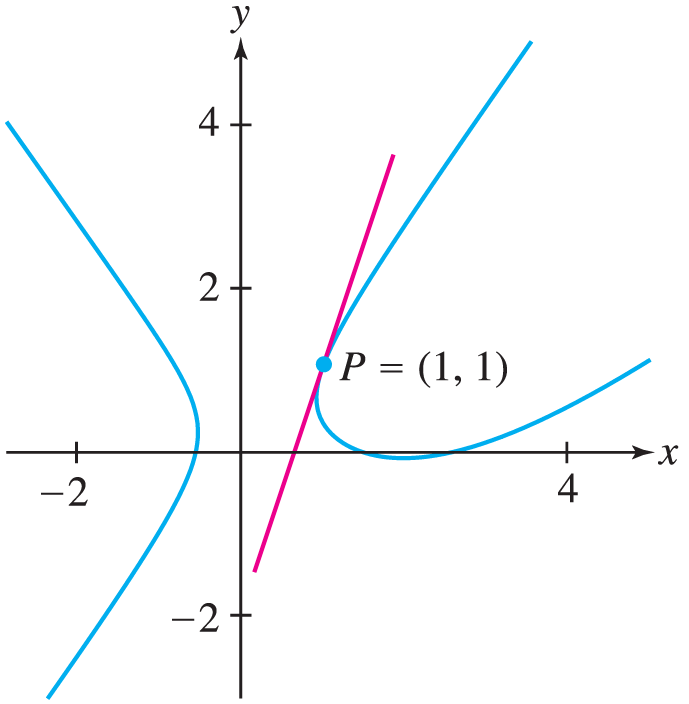
\includegraphics[width=2.5in]{10-26P_graph1.png}
        \vfill
\end{exercise}

\newpage

\section{Derivative of $\ln(x)$}
\label{LNX}

We can use implicit differentiation to compute the derivatives of \textbf{inverse functions}.\\
Recall that a function $f(x)$ is \textbf{1-to-1} if each function value $y = f(a)$ is hit exactly one time.
In this case, there is an inverse function $f^{-1}(x)$ such that
\[
        f^{-1}\big( f(x) \big) = x
\]
or equivalently that the left equation holds exactly when the right equation holds:
\[
        f(a) = b
        \qquad
        a = f^{-1}(b)
\]
\begin{example}
        The function $f(x) = e^x$ and $f^{-1}(x) = \ln(x)$ are inverse functions.
        More generally, $b^x$ and $\log_b(x)$ are inverse functions.
\end{example}

\begin{exercise}
        Compute the derivative of $y = \ln(x)$:
        \begin{enumerate}[(i)]
        \item Consider the equivalent equation $e^y = x$, and find $\dfrac{dy}{dx}$ using implicit differentiation.
                \vfill
        \item Substitute $x$ back in (\textit{what is $x$ equal to?}), so that the resulting function for $\dfrac{dy}{dx}$ is only in terms of $x$ (no $y$'s allowed!).
                \vfill
        \end{enumerate}
\end{exercise}

\begin{exercise}
        If $p(x) = \ln(x^2+1)$, find $p'(x)$.
        \vfill
\end{exercise}

\newpage

\section{Derivative of inverse trig functions}

In this section, we will follow a similar pattern as in \cref{LNX}.
However, to ``substitute $x$ back in'', we will need to use a \textit{geometric} understanding of the trig functions.

\begin{exercise}
        Compute the derivative of $y = \sin^{-1}(x)$:
        \begin{enumerate}[(i)]
        \item Consider the equivalent equation $\sin(y) = x$, and find $\dfrac{dy}{dx}$ using implicit differentiation.
                \vfill
        \item Draw a triangle with angle $y$, and label the sides in terms of $x$.
                \vfill
        \item Substitute $x$ back in (no $y$'s allowed!).
                \vfill
        \end{enumerate}
\end{exercise}


\end{document}
